\documentclass{article}

\usepackage{multirow}
\usepackage[utf8]{inputenc}
\usepackage{graphicx}
\usepackage{subfigure}

\begin{document}

\section{Association between the act of cross-posting and the drift of language usage of cross-posters}

The raw text of reddit posts (\texttt{body} field) were preprocessed, where HTML and other markup tags were removed. Then each post was tokenized into sentences, and each sentence was represented as a Bigram sequence of tokenized words. We performed two controlled computational experiments on the reddit text data processed as above using statistical language models.

In the first experiment, we investigated if the cross-posters' linguistic pattern in their HOME subreddit has manifested a significant change between the pre- and post-crossposting stage. As a control, we also considered the posts in the same subreddit that are from authors who never cross-posted. These posts were split into those that occurred in the first and second half of an author's lifespan. 

For each group, a fixed number (100,000) of sentences were bootstrapped (i.e. sampled with replacement) from the available text data (Table \ref{lm:tab1}), and for each sentence a log-transformed probability score was computed using Bigram language model (with Stupid backoff smoothing [CITE]). The Bigram model was trained on the text data from non-crossposters in the same subreddit (disjoint from those used in the test set), which contains the most posts compared to those from cross-posters, and represents the mainstream linguistic pattern of the subreddit. The total numbers of available sentences in the four groups from which the above test and training set were sampled are briefly summarized in Table \ref{lm:tab1}. 

As illustrated in Figure \ref{lm:fig1_1}, the linguistic pattern of both cross-posters and non-crossposters appeared to have drifted away from the mainstream of their HOME subreddit, when comparing the average of the log-probability of sentences in the early stage ("Pre-crossposting" and "First half") and late stage ("Post-crossposting" and "Second half") of an author's lifespan. Notice that the linguistic pattern of Feminism-to-MensRights cross-posters has drifted to a much larger degree compared to the Feminism non-crossposters. To evaluate the statistical significance of the observed difference in Feminism as well as the counterpart in MensRights, the procedure of training and test set sampling and language model building was repeated a hundred times, and for each repetition the delta ($\Delta_{cp}$) between "Post-crossposting" and "Pre-crossposting", and the delta ($\Delta_{Ncp}$) between "Second half" and "First half" was computed. The average of $\Delta_{cp}$ and the average of $\Delta_{Ncp}$ over the hundred repetitions was computed (Figure \ref{lm:fig1_2}). We found that, for Feminism, the average of $\Delta{cp}$ (0.1149) was found to be statistically different (t-test, p-value=$2.5e-184$) from that of $\Delta_{Ncp}$ (0.0182). However, for MensRights the means of two samples of delta (0.0325 and 0.0320) was not found to be statistically different (t-test, p-value=0.5524), which may suggest that Feminism-to-MensRights cross-posters appeared to be more radical or aggressive than the MensRights-to-Feminism cross-posters in terms of the change of linguistic patterns.




\begin{table}
    \centering
    \begin{tabular}{l l r r}\hline
        & & MensRights & Feminism\\
        & &            &         \\  
        \multirow{2}{*}{\textbf{Cross-poster}}      & "Pre-crossposting" & 820,850   & 77,460\\
                                                    & "Post-crossposting"  & 2,494,351 & 149,112\\
        \multirow{2}{*}{\textbf{Non-Crossposter}}   & "Fist half"      & 1,315,380 & 193,058\\
                                                    & "Second half"       & 1,391,906 & 242,324\\\hline
    \end{tabular}\
    \label{lm:tab1}
    \caption{Count of sentences of posts from cross-posters and non-crossposters. Bigram model was trained using 150,000 sentences from "First half" and "Second half", respectively, and 100,000 sentences were bootstrapped from the remaining in each of the four groups as the test set.}
\end{table}

\begin{figure}
    \centering
    \begin{subfigure}[b]{0.5\textwidth}
        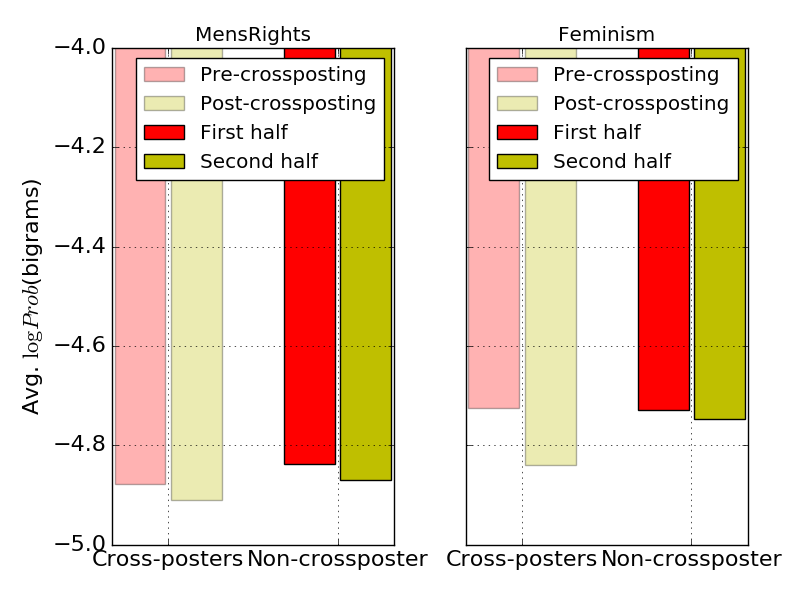
\includegraphics{images/LM_figure_1_1.png}
        \label{lm:fig1_1}
    \end{subfigure}
    \begin{subfigure}[b]{0.5\textwidth}
        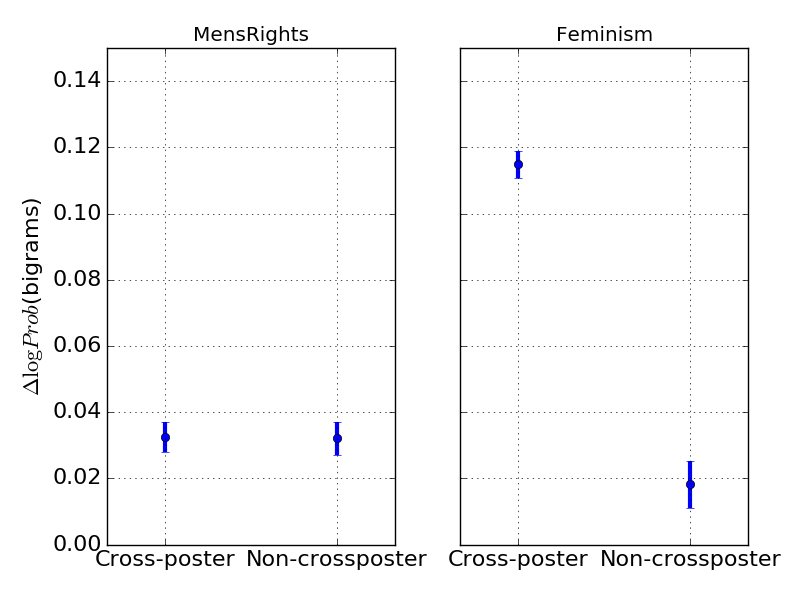
\includegraphics{images/LM_figure_1_2.png}
        \label{lm:fig1_2}
    \end{subfigure}[b]{0.5\textwidth}
    \caption{Association between cross-posting and drift of linguistic pattern}
\end{figure}


In the second experiment, we investigated whether the linguistic pattern of all authors (cross-posters and non-crossposters alike) has changed over the entire lifecycle of either subreddit. The posts were sorted in increasing order of the timestamp, and sorted list were split into 50 approximately equal-sized chunks. A log-probability was computed for each sentence in one chunk of data, using a Bigram model trained on the sentences from the remaining 49 chunks, and this was repeated for each of the 50 chunks. As a comparison, we considered an irrelevant subreddit "Cooking" on which this process was repeated. We plotted the average of the log-probability of sentences in each chunk as a function of the index (1 to 50). As shown in Figure \ref{lm:fig2}, for MensRights and Feminism the agreement of the local and the global linguistic pattern reached the maximum in the first half the lifecyle, and then decreases over time. In contrast, the linguistic pattern of the subreddit "Cooking" remains stable. It's also interesting to note that the evolution of the linguistic pattern in MensRights and Feminism appear to be correlated with each other ($\rho$ = 0.6636), in contrast to their correlation with the Cooking subreddit ($\rho$ = 0.3487 and 0.0445 for MensRights and Feminism). 

\begin{figure}
    \centering
    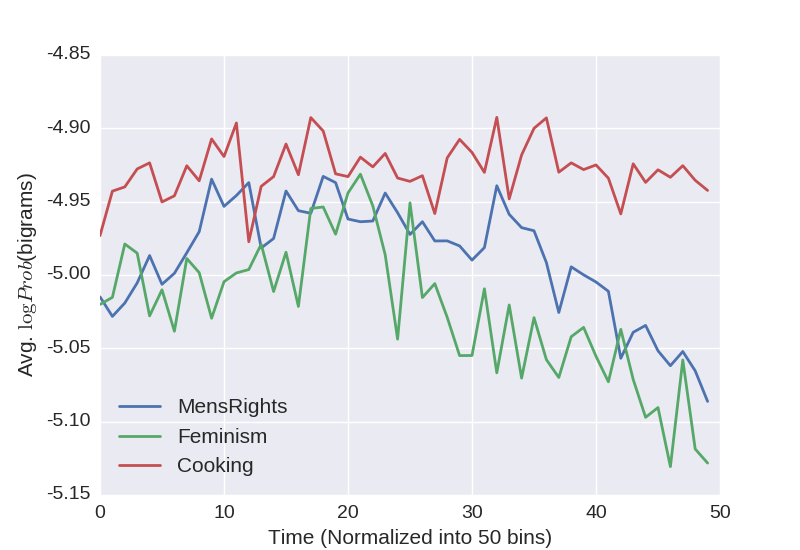
\includegraphics{images/LM_figure_2.png}
    \label{lm:fig2_1}
    \caption{The evolution of linguistic pattern over the lifecyle of subreddits}
\end{figure}



\end{document}